\section{Fallbeispiel: Der Zahllauf}\label{chap:paymentrun}

\nomenclature{IT}{Information Technology}
Im Bereich der Geschäftsanwendungen gibt es eine Reihe hochkomplexer Prozesse, die in der IT abgebildet werden.
Einer davon ist der sogenannte Zahllauf, bei dem sich der Anwender eine Liste von offenen Zahlungen erst vorschlagen lässt, den Vorschlag überprüft und anschließend die Bearbeitung durch das System veranlasst.
Dabei spielen insbesondere die Abhängigkeiten von Zahlungen, Lieferanten und Rabattverträgen eine wichtige Rolle, da sie im Idealfall in eine günstige Konstellation für das Unternehmen resultieren und dadurch Einsparungen bei den Ausgaben ermöglichen.

Aus diesem Grund hat die Implementierung des dazugehörigen Algorithmus viele Einflussfaktoren.
Zusätzlich erschweren große Relationen mit stark abgekürzten Namen von Feldern und Werten, die als Eingabe, Zwischenspeicher und Ausgabe dienen, das Erstellen einer daten- und performancebewussten Umsetzung.
Dies gilt besonders für domänenfremde Entwickler.
Umso wichtiger ist es, bereits frühzeitig in der Entwicklung relevante Testdaten zu nutzen, die auch Randfälle der Implementierung abdecken und Engpässe aufzeigen.
Dabei unterstützt die im Rahmen des Bachelorprojektes erstellte Web-IDE den Entwickler durch die in dieser Arbeit vorgestellten Ansätze zur Generierung von Testdatenvorschlägen.

In diesem Kapitel wird folgend exemplarisch die Implementierung des Zahllauf-Algorithmus mithilfe der Web-IDE vorgestellt.
Dabei steht die von Nutzereingaben geprägte Verarbeitung der Suche nach Belegen im Fokus.
Anschließend werden die vorgestellten Ansätze zur Testwertgenerierung anhand der Umsetzung des Fallbeispiels evaluiert.

\subsection{Implementierung des Algorithmus in der Web-IDE}

\begin{figure}[ht]
	\centering
  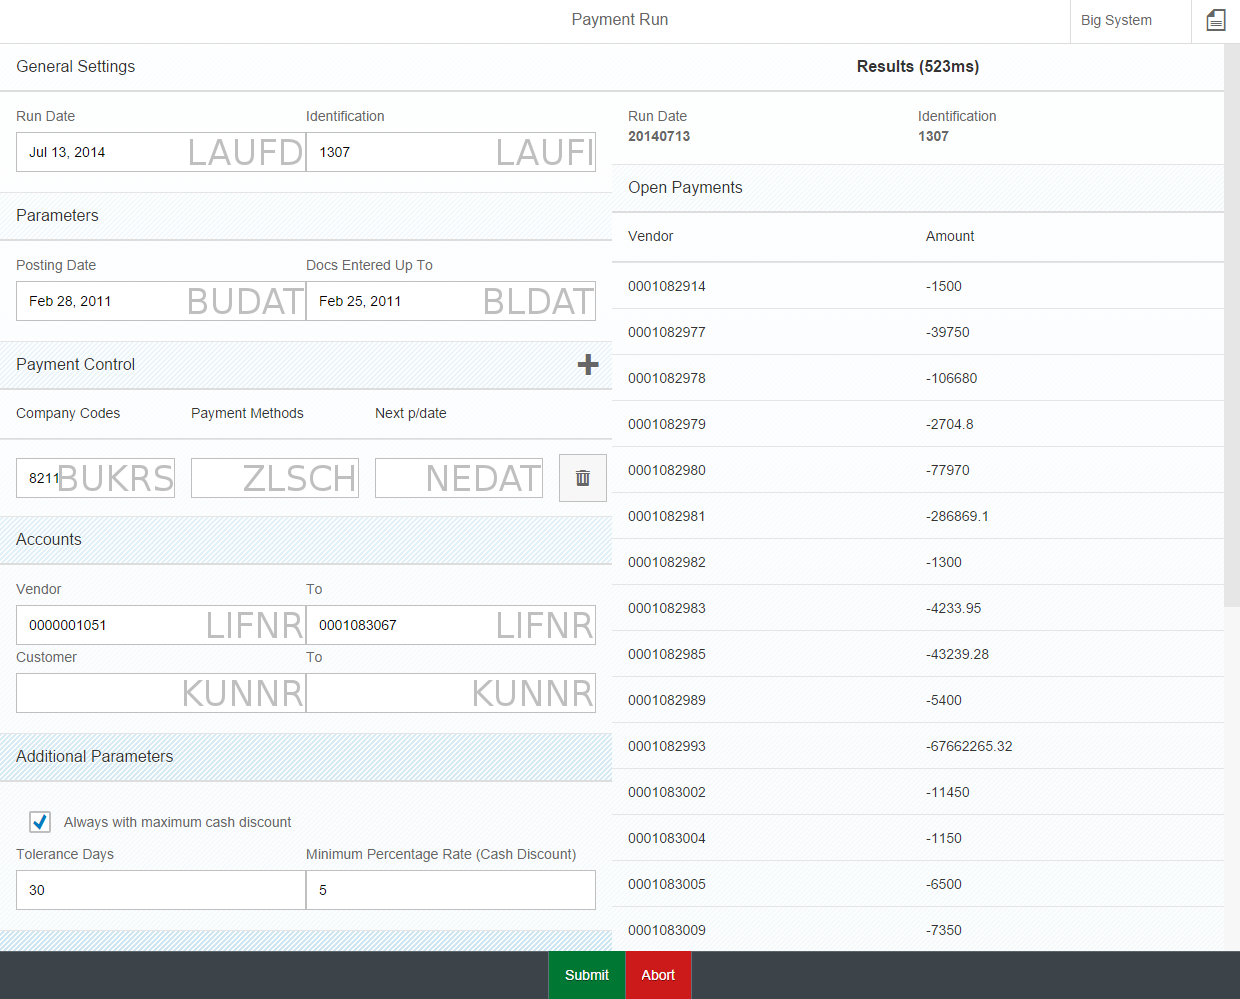
\includegraphics[width=1\textwidth]{figures/paymentrun.png}
	\caption{Eingabemaske des Zahllaufs}
	\label{fig:paymentrun}
\end{figure}

\nomenclature{UI}{User Interface}
Die in Abbildung \ref{fig:paymentrun} dargestellte Filtereingabemaske des Zahllaufs hat zwei Bestandteile.
Zum einen können allgemeine Parameter für die Suche festgelegt werden (z.B. das Ausführungsdatum (Run Date) und der Bereich der Lieferantennummern (Vendor)).
Zum anderen dient die Eingabe in Form einer Tabelle (Payment Control) zur Festlegung von zusammenhängende Suchkriterien.
Jede Zeile der Tabelle besteht aus einem Filter nach Buchungskreis (Company Codes), Zahlmethoden (Payment Methods) und dem nächsten Ausführungsdatum (Next p/date) und entspricht damit einem eigenen Suchlauf.

Für die Implementierung des Frontends wurde das UI-Framework OpenUI5\footnote{\url{http://sap.github.io/openui5/}} von SAP genutzt.
Der Fokus dieses Kapitels liegt jedoch auf der Backendimplementierung auf Basis der SAP XS-Engine\footnote{\url{http://help.sap.com/hana/SAP_HANA_XS_JavaScript_Reference_en/index.html}}.

\clearpage
Der Algorithmus des Zahllaufs besteht aus 5 Schritten:
   \begin{enumerate}
			\setlength{\itemsep}{0cm}%
			\setlength{\parskip}{0cm}%
      \item Parsen der JSON-Anfrage vom Frontend
			\item Selektion von Belegpositionen und Speicherung in der REGUP-Relation
			\item Berechnung von Zahldatum und Skonto
			\item Speicherung der Beleginformationen in der REGUH-Relation
			\item Senden einer JSON-Antwort
   \end{enumerate}

Die REGUP- und REGUH-Relationen dienen als datenbankinterne Zwischenspeicher für die ermittelten Ergebnisse.
Zur Selektion wird die Relation BSIK als materialisierte Sicht auf die BSEG-Relation genutzt.

Die Eingaben des Nutzers in der Filtermaske wirken sich insbesondere auf die Selektion der Belegpositionen aus.
Sie werden im ersten Schritt aus der JSON-Anfrage geparst (siehe Code-Beispiel \ref{lst:jsoninput} im Anhang) und fließen im Programmverlauf in das allgemeine SQL-Statement zur Selektion (siehe Code-Beispiel \ref{lst:regupgeneral} im Anhang) ein.

Code-Beispiel \ref{lst:laufi} zeigt exemplarisch wie die Projektion des SQL-Statements um das Ausführungsdatum (\texttt{LAUFD}) ergänzt wird.
Für das Identifikationsmerkmal (\texttt{LAUFI}) wird analog verfahren.

\begin{lstlisting}[caption={Ergänzung der Projektion um das Ausführungsdatum}, label={lst:laufi}, language=JavaScriptSQL]
	if(runDate){
			insertRegup += SQL SELECT @runDate AS LAUFD;
	} else {
			insertRegup += SQL SELECT '' AS LAUFD;
	}
\end{lstlisting}

Anschließend werden dem SQL-Statement das Buchungs- (\texttt{BUDAT}) und Erfassungsdatum (\texttt{BLDAT}) optional als Filter hinzugefügt (Code-Beispiel \ref{lst:budat}).

\begin{lstlisting}[caption={Einfügen zusätzlicher Filter}, label={lst:budat}, language=JavaScriptSQL]
	if(postingDate){
			insertRegup += SQL WHERE AND BSIK.BUDAT = @postingDate;
	}
	if(docsEnteredDate){
			insertRegup += SQL WHERE AND BSIK.BLDAT <= @docsEnteredDate;
	}
\end{lstlisting}

Für die Eingabe einer bzw. mehrerer Kundennummern (\texttt{KUNNR}) wird das bereits bekannte Code-Beispiel \ref{lst:newsql} aus Kapitel \ref{sec:sqlandsourcecode} genutzt und kann in leicht abgewandelter Form auch für Lieferantennummern (\texttt{LIFNR}) verwendet werden (Code-Beispiel \ref{lst:vendor}).

\begin{lstlisting}[caption={Unterscheidung zwischen Einzel- und Bereichsfilter}, label={lst:vendor}, language=JavaScriptSQL]
	if(vendor && !vendorTo ){
			insertRegup += SQL WHERE AND BSIK.LIFNR = @vendor;
	}
	if(vendor && vendorTo ){
			insertRegup += SQL WHERE AND BSIK.LIFNR BETWEEN @vendor
				AND @vendorTo;
	}
\end{lstlisting}

Das komplexeste Konstrukt der Eingabemaske ist die Tabelle für Kriterien zur Suche anhand von Buchungskreisen (\texttt{BUKRS}), Zahlmethoden (\texttt{ZLSCH}) und dem nächsten Ausführungsdatums (\texttt{NEDAT}) des Zahllaufs.
Die einzelnen Zellen einer Zeile bilden eine Konjunktion, wobei die Reihen untereinander jeweils disjunkt sind.
Die Komplexität entsteht durch die vielen Variationsmöglichkeiten der Eingabe.
So können Buchungskreise z.B. kommasepariert, mittels Klammern als Bereich oder beides kombiniert angegeben werden.
Die Zahlmethoden werden mit Großbuchstaben abgekürzt und aneinander gereiht um die Angabe mehrerer Methoden zuzulassen.

Die Verarbeitung der Nutzereingaben aus der Tabelle erfolgt dazu zeilenweise (siehe Code-Beispiel \ref{lst:paymentcontrol}).
Im ersten Schritt wird die Angabe der Buchungskreise geparst.
Zusammen mit den Zahlmethoden und nächsten Ausführungsdatum bildet sie einen Filter.
Die gebildeten Filter der einzelnen Zeilen werden als Disjunktion dem SQL-Statement angefügt wird.
Mit der anschließenden Ausführung des Statements ist der 2. Schritt des Algorithmus abgeschlossen.

Die nachfolgende Berechnung von Zahldatum und Skontobetrag erfolgt mithilfe einer SQLScript-Funktion.
Dies geschieht im selbe Zuge mit der Ermittlung und Speicherung der Beleginformationen in der REGUH-Relation.
Im letzten Schritt wird aus den Ergebnissen der REGUH-Relation die JSON-Antwort für den Anwender gebildet.
Sie umfasst das Ausführungsdatum und Identifikationsmerkmal, sowie eine Liste mit Lieferantennummern und Gesamtbeträgen.

Die vielen optionalen Eingaben durch den Anwender bestimmen das Aussehen, die Komplexität und die Laufzeit des untersuchten SQL-Statements.
In diesen Fällen ist es für Entwickler deshalb wichtig, relevante Testwerte zu haben, um früh in der Entwicklung Performance-Analysen zu ermöglichen.
Für das vorgestellte SQL-Statement werden dazu im folgenden Kapitel die Ansätze dieser Arbeit zur Vorschlagsgenerierung evaluiert.

\subsection{Evaluierung der vorgestellten Ansätze am Fallbeispiel}
% Die im Rahmen dieser Bachelorarbeit vorgestellten Ansätze zur Vorschlagsgenerierung von Testwerten werden in diesem Kapitel auf Basis des Fallbeispiels evaluiert.
%Zur Evaluation der vorgestellten Ansätze wurde ein vergleichendes Experiment auf Basis des Fallbeispiels durchgeführt.
Die vorgestellten Ansätze werden in diesem Kapitel anhand des Fallbeispiels auf ihre Ausführungsdauer und vorgeschlagenen Testwerten verglichen.
Als Grundlage dienen folgende mögliche Nutzereingaben zur Filterung der Ergebnisse des Zahllaufprogramms:

   \begin{itemize}
			\setlength{\itemsep}{0cm}%
			\setlength{\parskip}{0cm}%
      \item Buchungsdatum (\texttt{BUDAT})
      \item Belegdatum (\texttt{BLDAT})
			\item Lieferantennummer (\texttt{LIFNR})
			\item Zahlmethode (\texttt{ZLSCH})
			\item Buchungskreis (\texttt{BUKRS})
   \end{itemize}


%Die ermittelten Vorschläge nach dem in Kapitel \ref{chap:datacharacteristics} spezifizierten Verfahren sind in den Tabellen \ref{tab:paymentruntable1}, \ref{tab:paymentruntable2} und \ref{tab:paymentruntable3} dargestellt (siehe Anhang).
\begin{table}[ht!]
	\centering
	\scalebox{.73}{
	\begin{tabular}{ |c|c|c|c|c|c|c|c| }
		\cline{3-8}
		\multicolumn{2}{c|}{} & \multicolumn{6}{c|}{Häufigste Werte}\\
		\hline
		Spalte & Distinkte Werte & Wert & Vorkommen & Wert & Vorkommen & Wert & Vorkommen \\
		\hline
		BUDAT & 903 & \textbf{20110228} 	& 760 	& 20110221 	& 139 	& 20110224 	& 103 \\
		BLDAT & 933 & \textbf{20110216} 	& 177 	& 20101208 	& 124 	& 20101204 	& 118 \\
		LIFNR & 247 & \textbf{1051} 			& 3717 	& 2671 			& 1029 	& 1082993 	& 234 \\
		BUKRS & 9 	& \textbf{3451} 			& 4426 	& 8211 			& 816 	& 4101 			& 259 \\
		ZLSCH & 6 	& 					& 5739 	& T 				& 181 	& R 				& 10 \\
		\hline
	\end{tabular}
	}
	\caption{Ermittelte häufigste Werte der betrachteten Spalten}
	\label{tab:paymentruntable1}
\end{table}

Tabelle \ref{tab:paymentruntable1} zeigt die im ersten Schritt ermittelten drei häufigsten Werte für die betrachteten Spalten (entsprechend dem Verfahren in Kapitel \ref{chap:datacharacteristics}).
Naheliegend ist die Auswahl der Werte mit dem jeweils höchsten Vorkommen (in der Tabelle hervorgehoben).
Dies ist in diesem Fall nicht zielführend, da die so gewählte Konstellation von Werten keine Einträge in der Relation vorweist.

Mithilfe der adaptiven Erweiterung des Ansatzes (siehe Kapitel \ref{chap:adaptive}) wird deshalb die Kombination der Spalten betrachtet.
Tabelle \ref{tab:tupel} zeigt die vier Eingabetupel aus den so erstellten initialen Testdatensets.
%Die durch die initiale Erstellung der Testdatensets ermittelten zwei Eingabetupel sind in Tabelle \ref{tab:tupel} dargestellt.
%Die absteigende Sortierung anhand der Vorkommen der ermittelten Tupel und der gewählten Obergrenze von 50 resultieren in 2 gefunden Tupeln.

\begin{table}[ht]
	\centering
	\scalebox{.9}{
	\begin{tabular}{ |c|c|c|c|c|c|c| }
		\hline
		\texttt{BUDAT} & \texttt{BLDAT} & \texttt{LIFNR} & \texttt{ZLSCH} & \texttt{BUKRS} & Ergebnisse & Zeit (ms) \\
		\hline
		'20110228' & '20101208' & '0001082993' & ' ' & '8211' & 231 & 51,973 \\
		'20110228' & '20101204' & '0001082993' & ' ' & '8211' & 117 & 50,685 \\
		'20110221' & '20110216' & '0001063780' & ' ' & '3451' & 59 	& 49,280 \\
		'20110224' & '20110216' & '0001063780' & ' ' & '3451' & 51 	& 47,110 \\
		\hline
	\end{tabular}
	}
	\caption{Gefundene Tupel für Testdatensets inklusive Ausführungszeiten}
	\label{tab:tupel}
\end{table}



%\begin{figure}[h!]
%\centering
	%\begin{tikzpicture}
		%\begin{axis}[
				%axis lines=left,
				%width  = 1*\textwidth,
				%height  = 6cm,
				%ylabel={Anzahl distinkter Werte},
				%xlabel={Anzahl der Vorkommen in der Relation \texttt{BSIK}},
				%ymin=0.0,
				%xmin=0.0,
				%ymax=650.0,
				%xmax=780.0,
				%]
				%\addplot[only marks,color=blue,mark=square*,mark size=1pt] coordinates {
					%(1,630)
					%(2,102)
					%(3,25)
					%(4,19)
					%(5,10)
					%(6,6)
					%(7,1)
					%(8,3)
					%(10,1)
					%(11,3)
					%(13,1)
					%(16,1)
					%(17,1)
					%(19,2)
					%(20,1)
					%(21,2)
					%(22,2)
					%(25,1)
					%(27,2)
					%(28,1)
					%(29,4)
					%(31,2)
					%(32,4)
					%(33,4)
					%(34,4)
					%(35,5)
					%(36,6)
					%(37,5)
					%(38,6)
					%(39,4)
					%(40,6)
					%(41,5)
					%(42,3)
					%(43,4)
					%(44,4)
					%(45,2)
					%(46,1)
					%(47,1)
					%(48,1)
					%(49,3)
					%(50,1)
					%(52,3)
					%(54,2)
					%(55,2)
					%(56,2)
					%(59,1)
					%(66,1)
					%(103,1)
					%(139,1)
					%(760,1)
				%};
		%\end{axis}
	%\end{tikzpicture}
	%\caption{Verteilung der distinkten Werte in der Spalte \texttt{BUDAT}}
	%\label{fig:budatverteilung}
%\end{figure}
%
%Die Anzahl der gefunden Ergebnisse ist anhand der Verteilung der Daten innerhalb der jeweiligen Spalten erklärbar.
%Abbildung \ref{fig:budatverteilung} zeigt beispielhaft das Verhältnis der Anzahl distinkter Werte innerhalb der Spalte \texttt{BUDAT} zur Anzahl der Ausprägungen in der Relation.
%Besonders auffällig ist die starke Streuung.
%So gibt es beispielsweise 630 Werte, die jeweils nur in einem Datensatz der Relation vorkommen, wohingegen ein einziger Wert 760 Repräsentationen hat.
%In den weiteren vier betrachteten Spalten verhält sich die Verteilung analog.

Die Anzahl der gefunden Tupel kann anhand der Verteilung der Daten innerhalb der Relation erklärt werden.
Abbildung \ref{fig:combverteilung} zeigt das Verhältnis der Anzahl der distinkten Tupel zur ihrer Anzahl an Vorkommen in der Relation.

%Dies spiegelt sich auch in der Verteilung innerhalb der Kombination der Spalten \texttt{BUDAT}, \texttt{BLDAT}, \texttt{LIFNR}, \texttt{ZLSCH} und \texttt{BUKRS} wieder (siehe Abbildung \ref{fig:combverteilung}).


\begin{figure}[h]
\centering
	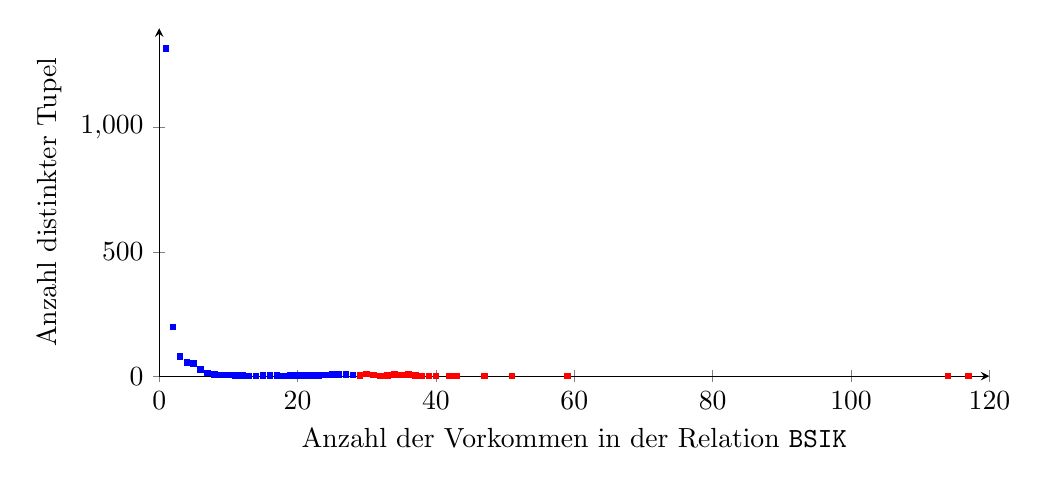
\begin{tikzpicture}
		\begin{axis}[
				axis lines=left,
				width  = 1*\textwidth,
				height  = 6cm,
				ylabel={Anzahl distinkter Tupel},
				xlabel={Anzahl der Vorkommen in der Relation \texttt{BSIK}},
				ymin=0.0,
				xmin=0.0,
				ymax=1400.0,
				xmax=120.0,
				scatter/classes={
					a={mark=square*,red},%
					b={mark=square*,blue}}
				]
				\addplot[scatter, only marks,mark size=1pt,scatter src=explicit symbolic] coordinates {
					(1,1318)	[b]
					(2,197)		[b]
					(3,79)		[b]
					(4,55)		[b]
					(5,50)		[b]
					(6,27)		[b]
					(7,13)		[b]
					(8,7)			[b]
					(9,4)			[b]
					(10,5)		[b]
					(11,2)		[b]
					(12,3)		[b]
					(13,1)		[b]
					(14,1)		[b]
					(15,2)		[b]
					(16,2)		[b]
					(17,2)		[b]
					(18,1)		[b]
					(19,2)		[b]
					(20,2)		[b]
					(21,2)		[b]
					(22,2)		[b]
					(23,3)		[b]
					(24,5)		[b]
					(25,7)		[b]
					(26,6)		[b]
					(27,6)		[b]
					(28,5)		[b]
					(29,3)		[a]
					(30,9)		[a]
					(31,5)		[a]
					(32,1)		[a]
					(33,3)		[a]
					(34,7)		[a]
					(35,4)		[a]
					(36,7)		[a]
					(37,2)		[a]
					(38,1)		[a]
					(39,1)		[a]
					(40,1)		[a]
					(42,1)		[a]
					(43,1)		[a]
					(47,1)		[a]
					(51,1)		[a]
					(59,1)		[a]
					(114,1)		[a]
					(117,1)		[a]
				};
		\end{axis}
	\end{tikzpicture}
	\caption{Verhältnis der distinkten Tupel zur Anzahl ihres Vorkommens}
	\label{fig:combverteilung}
\end{figure}

Besonders auffällig ist die starke Streuung.
So gibt es beispielsweise 1318 Tupel, die jeweils nur in einem Datensatz der Relation vorkommen, wohingegen zwei Tupel über 100 Repräsentanten haben.

Rot hervorgehoben ist der Anteil, der vom adaptiven Ansatz als initiale Eingabe genutzt wird.
Dies entspricht der absteigenden Sortierung anhand der Vorkommen sowie der festgelegten Obergrenze von 50 Tupeln.
Zusammen mit dem blauen Anteil ergibt dies in der Summe 1860 Tupel, was dem kompletten Eingaberaum entspricht.
Nur vier Tupel der betrachteten roten Menge ergeben bei Ausführung des Zahllaufprogramms ein Resultat mit mindestens einem Datensatz.
Dies sind die zuvor erwähnten Eingabetupel in Tabelle \ref{tab:tupel}.

\begin{figure}[h!]
\centering
	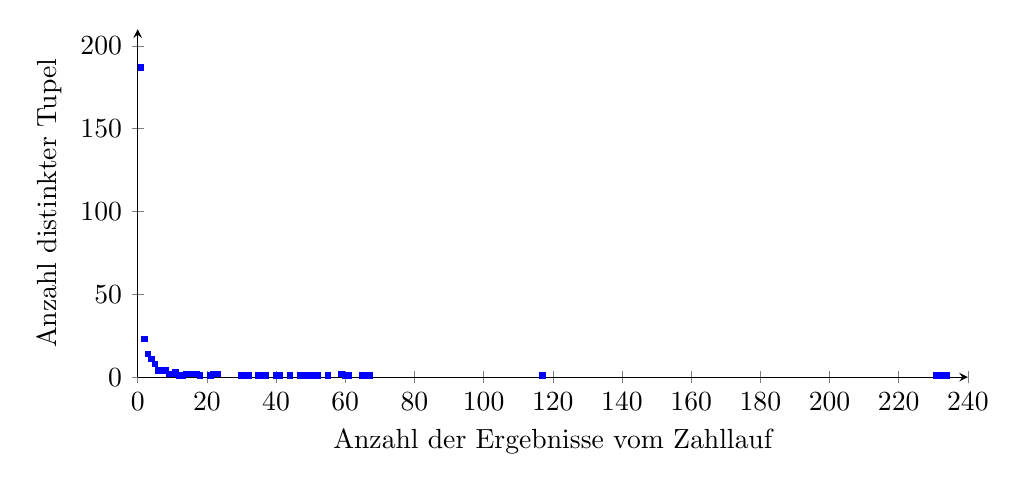
\begin{tikzpicture}
		\begin{axis}[
				axis lines=left,
				width  = 1*\textwidth,
				height  = 6cm,
				ylabel={Anzahl distinkter Tupel},
				xlabel={Anzahl der Ergebnisse vom Zahllauf},
				ymin=0.0,
				xmin=0.0,
				ymax=210.0,
				xmax=240.0,
				]
				\addplot[only marks,color=blue,mark=square*,mark size=1pt] coordinates {
					(1,187)
					(2,23)
					(3,14)
					(4,11)
					(5,8)
					(6,4)
					(7,4)
					(8,4)
					(9,2)
					(10,2)
					(11,3)
					(12,1)
					(13,1)
					(14,2)
					(15,2)
					(17,2)
					(18,1)
					(21,1)
					(22,2)
					(23,2)
					(30,1)
					(32,1)
					(35,1)
					(37,1)
					(40,1)
					(41,1)
					(44,1)
					(47,1)
					(49,1)
					(50,1)
					(51,1)
					(52,1)
					(55,1)
					(59,2)
					(60,1)
					(61,1)
					(65,1)
					(66,1)
					(67,1)
					(117,1)
					(231,1)
					(232,1)
					(233,1)
					(234,1)
				};
		\end{axis}
	\end{tikzpicture}
	\caption{Verteilung der 301 möglichen Eingabetupel für den Zahllauf}
	\label{fig:tupelbsikverteilung}
\end{figure}

Wird der komplette Eingaberaum für die Ausführung des Zahllaufprogramms genutzt, so haben nur 301 der 1860 Tupel ein Ergebnis mit mindestens einem Eintrag.
Dies entspricht einem Anteil von 16 \%.
Ihre Verteilung (siehe Abbildung \ref{fig:tupelbsikverteilung}) verhält sich analog zu der Beobachtung über den gesamten, potentiellen Eingaberaum (Abbildung \ref{fig:combverteilung}).
Nur fünf der Tupel haben über 100 Datensätze in ihren Resultaten, wohingegen 187 Tupel jeweils nur einen Datensatz umfassen.
Tabelle \ref{tab:tupel2} zeigt exemplarisch diese fünf Tupel mit den größten Ergebnismengen, wovon zwei den ermittelten Eingabetupeln in Tabelle \ref{tab:tupel} entsprechen.

\begin{table}[ht]
	\centering
	\scalebox{.85}{
	\begin{tabular}{ |c|c|c|c|c|c|c|c| }
		\hline
		Tupel & \texttt{BUDAT} & \texttt{BLDAT} & \texttt{LIFNR} & \texttt{ZLSCH} & \texttt{BUKRS} & Ergebnisse & Zeit (ms)\\
		\hline
        1 & '20110228' & '20101227' & '0001082993' & ' ' & '8211' & 234 & 52,317 \\
        2 & '20110228' & '20101220' & '0001082993' & ' ' & '8211' & 233 & 51,689 \\
        3 & '20110228' & '20101213' & '0001082993' & ' ' & '8211' & 232 & 50,240 \\
        \textbf{4} & \textbf{'20110228'} & \textbf{'20101208'} & \textbf{'0001082993'} & \textbf{' '} & \textbf{'8211'} & \textbf{231} & \textbf{49,917} \\
        \textbf{5} & \textbf{'20110228'} & \textbf{'20101204'} & \textbf{'0001082993'} & \textbf{' '} & \textbf{'8211'} & \textbf{117} & \textbf{49,280} \\
		\hline
	\end{tabular}
	}
	\caption{Eingabetupel mit den meisten Ergebnissen}
	\label{tab:tupel2}
\end{table}

Im Weiteren wird deshalb der Einfluss der gewählten Obergrenze auf die Anzahl der ermittelten Eingabetupel mit mindestens einem Ergebnisdatensatz untersucht.
%TODO: Es wird vermutet, dass die gewählte Obergrenze an zu betrachtenden Tupeln die Anzahl der ermittelten Eingabetupel beeinflusst.
Dazu wird die Grenze stufenweise erhöht und mit der benötigten Laufzeit sowie der Menge an ermittelten Tupeln verglichen.

Die Messergebnisse (siehe Tabelle \ref{tab:tupel3}) zeigen, dass mit steigender Betrachtung von Tupeln auf der einen Seite die Anzahl der gefundenen Eingabetupel für Testdatensets steigt, auf der anderen Seite jedoch auch die Laufzeit der Analysen wächst.
Aufgrund dessen ist es in Erwägung zu ziehen, dem Entwickler die Möglichkeit der manuellen Festlegung der Obergrenze zu geben.
Er könnte so das Verhältnis zwischen dem Maximum an initial ermittelten Testdatensets und der für ihn vertretbaren Laufzeit selbst festlegen.
Die optimale Parameterwahl bedarf dabei weiteren Untersuchungen der Beziehung zwischen der Anzahl der betrachteten Spalten, der Verteilung der Daten und der Laufzeit der Berechnungen.

\begin{table}[b]
	\centering
	\scalebox{.85}{
	\begin{tabular}{ |c|c|c|c|c|c|c|c| }
		\hline
		Obergrenze 	& Anzahl gefundener Tupel & Laufzeit (sek)\\
		\hline
        50 			& 4 											& 0,06 \\
        100 		& 5												& 0,12 \\
        500 		& 50 											& 0,59 \\
        1000 		& 81 											& 1,14 \\
        1500 		& 236 										& 1,77 \\
				2000 		& 301 										& 2,25 \\
		\hline
	\end{tabular}
	}
	\caption{Auswirkung der Wahl der Obergrenze auf Eingabetupel und Laufzeit}
	\label{tab:tupel3}
\end{table}

Aus Gründen der Einfachheit und Geschwindigkeit des Feedbacks für den Entwickler wird die adaptive Lösung mit fester Obergrenze für den Einsatz in der Web-IDE favorisiert.
Sie ermöglicht es, auf Grundlage der explorativen Erweiterung die Menge der initial ermittelten Testdatensets kontinuierlich zu erweitern und stellt somit ein Kompromiss aus Laufzeit und Menge an Testdaten dar.







%
%
%
%
%
%TODO: WO?? Überrebiten
%Vergleicht man die ermittelten Testdatensets...
%Vergleicht man die ermittelten Testdatensets mit den initial vorgeschlagenen häufigsten Werten der einzelnen Spalten, fällt auf, dass die Werte des Buchungsdatums, der Lieferantennummer, der Zahlmethode und des Buchungskreises konstant bleiben und nur das Belegdatum in seinem Wert variiert.
%Des Weiteren ist zu beobachten, dass alle Werte aus den ermittelten Listen der häufigsten Werte stammen.
%Dies lässt sich über die Verteilung der Daten, welche in den Abbildungen \ref{fig:budatverteilung} bis \ref{fig:zlschverteilung} (siehe Anhang) dargestellt sind, erklären.
%Die Grafiken zeigen das Verhältnis der Anzahl distinkter Werte innerhalb einer Spalte zur Anzahl der Ausprägungen in den Einträgen der Relation.
%TODO: Referenz Abb.
%Beispielsweise haben 630 distinkte Werte in der Spalte \texttt{BUDAT} nur jeweils einen Eintrag, wohingegen ein einziger Wert 760 Repräsentationen in der Relation hat.
%TODO: Was heißt das? ...und das bedeutet
%
%TODO: Was zeigt sich da?
%Dies zeigt sich besonders in den Abbildungen \ref{fig:budatverteilung} (\texttt{BUDAT}), \ref{fig:bldatverteilung} (\texttt{BLDAT}) und \ref{fig:lifnrverteilung} (\texttt{LIFNR}).
%Es wird deutlich, dass die Mehrheit der gefundenen distinkten Werte in den Spalten meist nur in einem Eintrag der Relation genutzt wird.
%TODO: Was heißt das für meine Vorschläge?
%Dem gegenüber stehen wenige Ausnahmen, die eine hohe Anzahl von Repräsentationen innerhalb der Relation aufweisen.
%Dies zeichnet sich auch in den vorgeschlagenen Werten um den Median ab (Tabelle \ref{tab:paymentruntable3}), bei dem die ermittelten Werte für die Spalten \texttt{BUDAT}, \texttt{BLDAT} und \texttt{LIFNR} auch dort nur einen Eintrag vorweisen.
%TODO: Was heißt das? ..das bestätigt , diese legt nahe, ...das fehler gering tsind
%
%Generell fällt auf  das die Spalten strueung hinstichltihc der anzahl
%viele werte nur einmal ...
%zeigt sich in den spalten
%es ist auch hier zu erkennen...
%Ebenso zeigen die Verteilung der Daten in den Spalten \texttt{BUKRS} und \texttt{ZLSCH} (Abbildung \ref{fig:bukrsverteilung} und \ref{fig:zlschverteilung}) eine deutlich Spaltung.
%So ist zu erkennen, dass jeweils ein Wert im Großteil der Einträge in der Relation genutzt wird und somit die anderen Werte nur wenige Ausprägungen haben.
%TODO: Aufgrund der wenigen distinkten Werte ergibt dies eine Gerade in der Darstellung.
%
%TODO: Der Brute-Force- Ansatz, der über eine PErmutation...
%Ein Vergleich mit allen möglichen Wertkombinationen würde die Berechnung einer Permutation über alle Listen der distinkten Werte der fünf betrachteten Spalten erfordern.
%Aufgrund der Größe der einzelnen Listen (\texttt{BUDAT} 903, \texttt{BLDAT} 933, \texttt{LIFNR} 247, \texttt{ZLSCH} 6, \texttt{BUKRS} 9) ergäbe sich in der Gesamtsumme ein Liste mit über 11 Milliarden Einträgen.
%Des Weiteren hat nur ein Bruchteil dieser Kombinationen mindestens einen Repräsentanten in der Datenbank.
%TODO:was heißt das?
%In der Annahme, dass die Berechnung der Analyse pro Listeneintrag 10ms braucht, würde dies zur einer Berechnungszeit von über 3 Jahren führen.
%Dieser Ansatz scheidet daher für die weiteren Betrachtungen dieser Analyse aus.
%
%TODO: Die folgenden Vergelcieh beziehen sich daher auf...
%Aus diesem Grund fokussiert sich das Experiment auf den Vergleich der Ergebnisse folgender Ansätze:
%
   %\begin{enumerate}
      %\item Adaptiver Algorithmus mit fester Obergrenze (50)
      %\item Adaptiver Algorithmus ohne feste Obergrenze
			%\item Permutation der ermittelten häufigsten, seltensten und mittleren Werte der Spalten
   %\end{enumerate}
%
%TODO: Zuncähst,... warum 5, warumd ie meisten?
%Dazu wird ermittelt, welcher der Ansätze die meisten der 5 Tupel mit den größten Ergebnismengen zurückgibt (zu sehen in Tabelle \ref{tab:tupel2}).
%Dies wird zusätzlich in Beziehung zu der Anzahl der betrachteten Tupel und der Laufzeit der Ermittlung betrachtet.
%
%\begin{table}[h]
	%\centering
	%\scalebox{.85}{
	%\begin{tabular}{ |c|c|c|c|c|c|c|c| }
		%\hline
		%Tupel & \texttt{BUDAT} & \texttt{BLDAT} & \texttt{LIFNR} & \texttt{ZLSCH} & \texttt{BUKRS} & Ergebnisse & Zeit (ms)\\
		%\hline
        %1 & '20110228' & '20101227' & '0001082993' & ' ' & '8211' & 234 & 52,317 \\
        %2 & '20110228' & '20101220' & '0001082993' & ' ' & '8211' & 233 & 51,689 \\
        %3 & '20110228' & '20101213' & '0001082993' & ' ' & '8211' & 232 & 50,240 \\
        %4 & '20110228' & '20101208' & '0001082993' & ' ' & '8211' & 231 & 49,917 \\
        %5 & '20110228' & '20101204' & '0001082993' & ' ' & '8211' & 117 & 49,280 \\
		%\hline
	%\end{tabular}
	%}
	%\caption{Eingabetupel mit den meisten Ergebnissen}
	%\label{tab:tupel2}
%\end{table}
%
%TODO: was sehe ich? tupel als referenz zum treffen, tabelle 4
%Die Messungen für die drei genannten Ansätze (siehe Tabelle \ref{tab:tupel3}) zeigen, dass die Einschränkung durch die Obergrenze den Umfang der gefundenen Tupel reduziert.
%TODO: wie reduziert? substantiell
%Die Betrachtung der Permutation ergibt zwar ein Tupel mehr, benötigt aber über eine halbe Minute für die Bestimmung, da mehr als 30.000 Tupel getestet werden.
%TODO: was passower wenn ich nur 2 oder 3 habe?
%
%\begin{table}[h]
	%\centering
	%\scalebox{.75}{
	%\begin{tabular}{ |c|c|c|c|c|c|c|c|c| }
		%\cline{2-8}
		%\multicolumn{1}{c|}{} & Tupel 1 & Tupel 2 & Tupel 3 & Tupel 4 & Tupel 5 & Getestete Tupel & Laufzeit (sek)\\
		%\hline
        %mit Obergrenze &  &  &  & X & X & 50 & 0,058 \\
        %ohne Obergrenze & X & X & X & X & X & 1.860 & 2,239 \\
        %Permutation & X &  &  & X & X & 30.618 & 34,352 \\
		%\hline
	%\end{tabular}
	%}
	%\caption{Vergleich der evaluierten Ansätze}
	%\label{tab:tupel3}
%\end{table}
%
%TODO: Wass?
%Der Grund für die vollständige Abdeckung der Tupel der Variante ohne Obergrenze liegt in der Ermittlung der zu testenden Tupel.
%Die 1.860 bestimmten Tupel entsprechen allen distinkten Konstellationen der Werte der betrachteten Spalten.
%Davon haben insgesamt nur 301 mindestens eine Ergebniszeile beim Ausführen des Programms, was einer Abdeckung des kompletten Eingaberaums entspricht.
%TODO: mehr erklären!
%Die Festlegung einer Obergrenze entspricht also einer Einschränkung auf einen Unterraum.
%Die Verteilung der 301 Tupel (siehe Abbildung \ref{fig:tupelverteilung}) macht deutlich, dass der Großteil der Eingabekonstellationen nur eine Ergebniszeile aus der Datenbank zurückgibt (187 Tupel) und nur wenige Tupel eine größere Ergebnismenge abrufen (5 Tupel mit über 150 Ergebnissen, erfasst in Tabelle \ref{tab:tupel2}).
%Dies spiegelt die zuvor betrachtete Verteilung der Daten innerhalb der einzelnen Spalten wieder.
%TODO: siehe irgendwas
%
%Aufgrund dessen ist es in Erwägung zu ziehen, dem Entwickler die Möglichkeit der manuellen Festlegung einer Obergrenze zu geben.
%TODO: was kann er damit machen?
%Dies bedarf weiterer Untersuchungen im Hinblick auf die Beziehung zwischen der Anzahl der betrachteten Spalten, dem Umfang an distinkten Werten und der Laufzeit der Berechnungen.
%TODO: nicht dies, die optimale parameterwahl, die möglichkeit?
%
%\begin{figure}[ht]
%\centering
	%\begin{tikzpicture}
		%\begin{axis}[
				%axis lines=left,
				%width  = 1*\textwidth,
				%height  = 6cm,
				%%symbolic x coords={1,2,3,4,5,6,7,8,9,10,11,12,13,14,15,15,18,21,22,23,30,32,35,37,40,41,44,47,49,50,51,52,55,59,60,61,65,66,67,117,231,232,233,234},
				%%xtick=data,
				%%enlarge x limits=0.05,
				%%bar width=5pt,
				%%ybar,
				%ylabel={Eingabetupel},
				%xlabel={Anzahl der Ergebniszeilen},
				%ymin=0.0,
				%ymax=200.0,
				%xmax=250.0,
				%]
				%%\addplot[ybar,fill=light-gray] coordinates {
				%\addplot[color=red,mark=x] coordinates {
						%(1,187)
						%(2,23)
						%(3,14)
						%(3,14)
						%(4,11)
						%(5,8)
						%(6,4)
						%(7,4)
						%(8,4)
						%(9,2)
						%(10,2)
						%(11,3)
						%(12,1)
						%(13,1)
						%(14,2)
						%(15,2)
						%(15,2)
						%(18,1)
						%(21,1)
						%(22,2)
						%(23,2)
						%(30,1)
						%(32,1)
						%(35,1)
						%(37,1)
						%(40,1)
						%(41,1)
						%(44,1)
						%(47,1)
						%(49,1)
						%(50,1)
						%(51,1)
						%(52,1)
						%(55,1)
						%(59,2)
						%(60,1)
						%(61,1)
						%(65,1)
						%(66,1)
						%(67,1)
						%(117,1)
						%(231,1)
						%(232,1)
						%(233,1)
						%(234,1)
				%};
		%\end{axis}
	%\end{tikzpicture}
	%\caption{Verteilung der Anzahl von Ergebniszeilen der Eingabetupel}
	%\label{fig:tupelverteilung}
%\end{figure}
%
%TODO: aus gründen x,y,z wird die adapttive Lösung für den Einsatz in der Web-IDE favorisiert...
%Die derzeitige adaptive Lösung ermöglicht es, auf Grundlage der mit einer Obergrenze ermittelten initialen Testdatensets durch explorative Erweiterung den erfassten Datensatz zu ergänzen.
%TODO: 2 Sätze

%\begin{table}[h]
	%\centering
	%\scalebox{.9}{
	%\begin{tabular}{ |c|c|c|c|c|c|c| }
		%\hline
		%\texttt{BUDAT} & \texttt{BLDAT} & \texttt{LIFNR} & \texttt{ZLSCH} & \texttt{BUKRS} & Ergebnisse & Zeit (ms)\\
		%\hline
		%\textbf{'20110228'} & \textbf{'20110216'} & \textbf{'0001082993'} & \textbf{' '} & \textbf{'8211'} & \textbf{234} & \textbf{52,317} \\
		%'20110228' & '20101220' & '0001082993' & ' ' & '8211' & 233 & 51,689 \\
		%'20110228' & '20110216' & '0001082993' & ' ' & '8211' & 232 & 50,240 \\
		%\textbf{'20110228'} & \textbf{'20101213'} & \textbf{'0001082993'} & \textbf{' '} & \textbf{'8211'} & \textbf{231} & \textbf{49,917} \\
		%\textbf{'20110228'} & \textbf{'20101204'} & \textbf{'0001082993'} & \textbf{' '} & \textbf{'8211'} & \textbf{117} & \textbf{49,280} \\
		%\hline
	%\end{tabular}
	%}
	%\caption{Gefundene Tupel für Testdatensets}
	%\label{tab:tupel2}
%\end{table}

%Die Messergebnisse zeigen, dass 3 der 5 Kombinationen von Eingabewerten mit den höchsten Ergebnismengen und Laufzeiten durch die vorgestellten Ansätze vorgeschlagen wurden (in Tabelle \ref{tab:tupel2} dick hervorgehoben).
%Im Vergleich mussten dazu jediglich
%Zusätzlich kann die adaptive Variantedurch exploratives Probieren weitere Testwerte durch den Entwickler dem ermittelten Datensatz ergänzen.
